% Generated by scripts/write_paper.py; do not edit (edit the template / figures/captions.md and rerun).
\begin{figure}[tbhp]
\centering
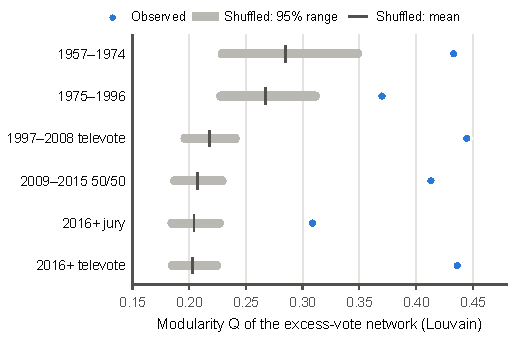
\includegraphics[width=\linewidth]{fig1_modularity}
\caption{Modularity of the excess-vote network, observed and under a shuffle null, per era. Each row is one network: one per era (1957–1974, 1975–1996, 1997–2008, 2009–2015) and, for 2016–2026, separate jury and televote networks. Nodes are countries; an edge joins two countries whose votes for each other (both directions pooled, at least 5 votes) have a positive mean excess, weighted by that mean (18–45 nodes per network). Blue dots: modularity Q of the best of five Louvain runs on the observed network. Grey bars: middle 95\% of Q over 1,000 networks in which each voter's points were randomly re-assigned among the entries it rated in the same year, round and vote type (same Louvain procedure); vertical tick: mean of the shuffled networks.}
\label{fig:fig1}
\end{figure}

\begin{figure}[tbhp]
\centering
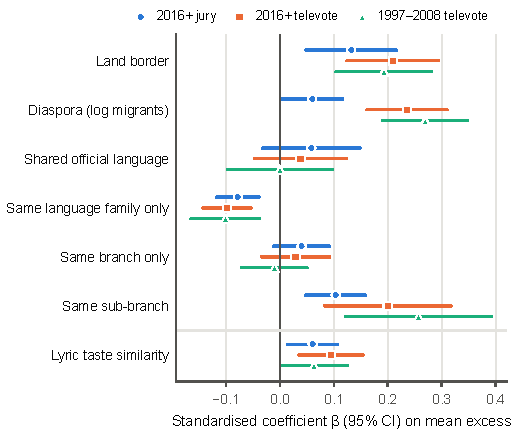
\includegraphics[width=\linewidth]{fig2_coefficients}
\caption{Standardised regression coefficients for the mean signed excess a voting country gives a receiving country. One OLS model per vote type: 2016–2026 jury (blue circles), 2016–2026 televote (orange squares) and 1997–2008 televote (green triangles); one observation per directed country pair with at least 5 votes (n = 1,537, 1,537 and 1,257 pairs). Outcome and predictors are z-scored within each model. Language family, branch and sub-branch enter as one category (deepest shared Glottolog level; reference: different families). Lyric taste similarity is the cosine similarity between the receiver's song and the voter's points-weighted lyric profile from other years, built from the same vote type. Lines: 95\% confidence intervals from standard errors clustered two-way by voting and receiving country (negative eigenvalues of the covariance set to zero, same estimator in all models). The horizontal rule separates the lyric term from the friendship terms.}
\label{fig:fig2}
\end{figure}

\begin{figure*}[tbhp]
\centering
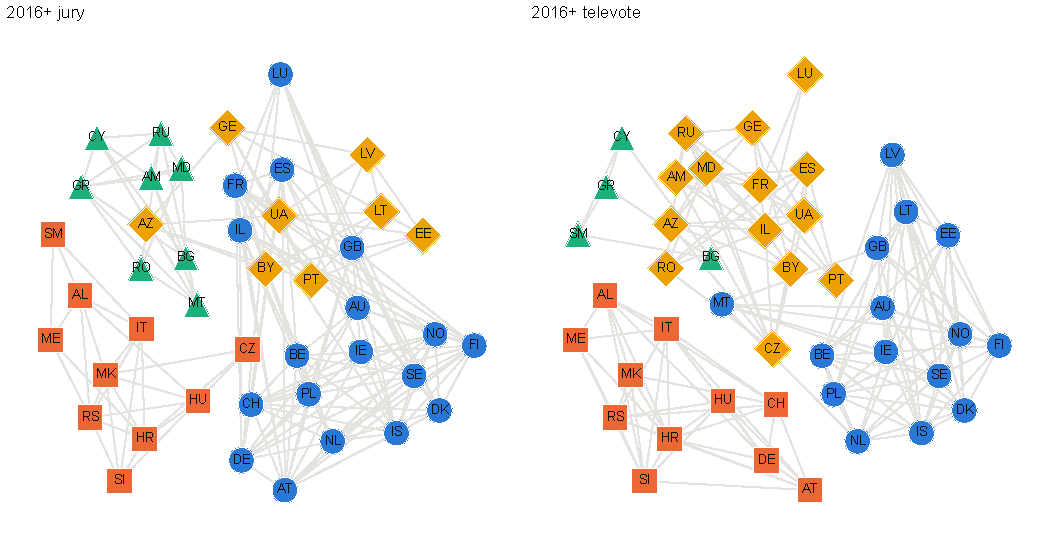
\includegraphics[width=0.9\textwidth]{fig3_communities}
\caption{Louvain communities of the 2016–2026 excess-vote networks for jury votes (left) and televotes (right), 44 countries and 4 communities in each. Marker colour and shape show community membership; a community in the televote panel gets the colour and shape of the jury community it overlaps most (one-to-one matching on the Jaccard index). Node positions are the same in both panels (one force-directed layout of the two networks combined, all edges). Grey lines: the disparity-filter backbone \cite{serrano2009backbone} of each network at $\alpha$ = 0.05, i.e. pairs (positive mean excess, both directions pooled, at least 5 votes) whose share of at least one country's positive excess is larger than a random split over its partners would give; 23 of 404 jury and 29 of 333 televote edges are kept. Solid: both countries in the same community; dashed: different communities. Labels are ISO 3166 country codes.}
\label{fig:fig3}
\end{figure*}
